%% Last modified: Time-stamp: <2011-06-22 22:57:53 (srdbadmin)>
\documentclass[letterpaper,review,authoryear,12pt]{myelsarticle}
\usepackage{amssymb}
\usepackage{pdflscape}
\usepackage{longtable}
\usepackage{graphicx}
\usepackage{paralist}
\usepackage{comment}
\usepackage{color}
\usepackage[left=3cm,top=3cm,right=3cm,bottom=3cm,nohead]{geometry}
\usepackage{booktabs}
\usepackage{url}
\usepackage[none]{hyphenat}  %% no hyphenation, to facilitate conversion to Word
\usepackage{microtype} %% no ligature, to facilitate conversion to Word
\DisableLigatures{encoding = *, family = * }
\usepackage{appendix}

\begin{document}

\begin{frontmatter}
\title{Database contents for the Abstract, Results, Tables and Figures of the Fish and Fisheries paper 2011 resubmission}
\date{\today}
\end{frontmatter}

%\newpage
\section*{Abstract}

Data used to assess the status of individual fish stocks varies from
very little information on many of the world's artisanal fisheries, to
commercial landings, research surveys, and sophisticated population
dynamics models that integrate many sources of information.  Previous
evaluations of the state of global fisheries have used catch data,
which may be poor proxies for fish stock abundances. A global
compilation of stock assessment data in the mid-1990s enabled
substantial syntheses of stock status; however its focus was on
stock-recruitment relationships and it is now 15 years out of date. To
facilitate contemporary syntheses, we have assembled a new database,
the RAM Legacy Database, of the most intensively studied commercially
exploited marine fish stocks, including time series of total biomass,
spawner biomass, recruits, fishing mortality, and catch; reference
points; and ancillary information on the life history, management, and
assessment methods for each stock.  Here, we present the first
overview of this database and use it to evaluate the knowledge-base
for assessed marine species.  Assessments were assembled for
323 stocks (287 fish species
representing 45 families, and
36 invertebrate species representing
12 families), including 8 of the world's 10
largest fisheries. Assessments were obtained from 18 national and
international management institutions, with most coming from North
America, Europe, Australia, New Zealand and the high seas.  Overall,
58\% of stocks are below $B_{msy}$, and 30\% have exploitation levels above
$U_{msy}$.  Assessed marine fish stocks comprise a relatively small
proportion of harvested taxa (24\%), and an even smaller proportion of
marine fish biodiversity (1\%).


%Globally, stock assessments were found
%for 323 stocks (287 species
%of fishes representing 45 families and
%36 species of invertebrates representing
%12 families), from 18
%national and international
%management institutions.

\noindent Keywords: marine fisheries, meta-analysis, population dynamics models, relational database, stock assessment, synthesis.

%with XX\% coming from north temperate regions (North
%Atlantic, North Pacific)
%\noindent Keywords: marine fisheries, meta-analysis, population dynamics models, relational database, stock assessment, synthesis.
%\newpage

%  Geographic differences in assessment
%methods show that Statistical Catch at Age (SCA) models are widely
%used by the west coast of the U.S. (XX percent of assessments),
%regional fishery management organizations in the Pacific (XX percent
%of assessments), and New Zealand (XX percent of assessments); the east
%coast of the U.S. is transitioning from Virtual Population Analysis
%(VPA) to SCA (XX percent of assessments conducted since 2000 have used
%SCA); while VPA is still the dominant assessment
%technique in western Europe (XX percent of assessments).

\section*{Results}
\subsection*{Summary}
\noindent
Total number of proper stocks assessments: 331, from 295 marine fish populations and 36
invertebrate populations.

\subsection*{Taxonomy}
\noindent

Number of species in FishBase: 12339 (from 54 orders) \\
Number of species in SAUP: 925 (from 36 orders)\\
Number of species in RAM Legacy: 163 (from 58 families and 20 orders) \\
RAM Legacy contains 18\% of SAUP and 1\% of FishBase species\\
Top 5 taxonomic orders in RAM Legacy: Gadiformes (n=70), Perciformes (n=65), Pleuronectiformes (n=53), Scorpaeniformes (n=41), Clupeiformes (n=36) \\

\subsection*{Timespan}
\noindent
Number of assessments with catch timeseries: 313.\\
Number of assessments with recruitment timeseries: 274.\\
Number of assessments with spawning stock biomass timeseries: 280.\\

Together these comprise time series of
catch/landings for 313 stocks (95\%),
SSB estimates for 280 stocks (85\%), and recruitment estimates for
274 stocks (83\%).

The median lengths of catch/landings, SSB, and recruitment timeseries
were 39, 34, and 33
years, respectively.  The time period covered by 90\% of assessments
is: catch/landings (1966-2007), SSB
(1972-2007), recruitment (1971-2006), while that
covered by 50\% of assessments is: catch/landings
(1983-2004), SSB (1985-2005), recruitment
(1984-2003)
 
\subsection*{Assessment methodologies and reference points}
\noindent
The three most common assessment methods were
Statistical catch-at-age/length models (n=169), Virtual Population Analyses (n=92) and
Biomass dynamics model (n=45). Regionally, Virtual Population Analysis
(VPA) is still the most common assessment model for European stocks
(71\% of 63 assessments),
Canada (56\% of 26
assessments) and Argentina (83\% of
6 assessments), whereas statistical catch-at-age
and -length models are more common for the United States
(67\% of 138 assessments),
Australia (82\% of 17
assessments) and New Zealand (76\% of
29 assessments).

Biomass- or exploitation-based reference points were available for
262 (82\%) and
224 (69\%)
assessments, respectively.

\subsection*{Stock status}
\noindent

MSY-related reference points were avaialble for
113 stocks
(3 invertebrates) and estimated
for 102 additional stocks
(15 invertebrates), for a total of
215 stocks.

Of the
215 stocks presented in
the fried egg, 113 and
102 of the biomass reference points and
83 and
132 of the exploitation reference
points come from assessments and from surplus production model fits,
respectively.

To identify potential biases arising from using BRPs
derived from surplus production models we computed a contingency table
of status classification for stocks that have both assessment- and
Schaefer-derived BRPs (Table S2). Surplus production models correctly
classified ratios of current biomass to BRPs in
77\% of cases (for 60
of 78 assessments) and 64\%
of cases for exploitation BRPs (for 28 of
44 assessments).

Overall, 59\% of stocks are estimated
to be below their biomass-related MSY BRP, that is $B_{curr}<B_{msy}$,
and 31\% are estimated to be above
their exploitation-related MSY BRP, $U_{curr}>U_{msy}$
(n=215 stocks total.
Of the stocks for which biomass is currently estimated to be below
$B_{msy}$, 54\% have had their
exploitation rate reduced below $U_{msy}$, suggesting potential for
recovery. The remaining
46\% of these stocks however,
still have excessive exploitation rates. On a positive note,
41\% of all stocks are estimated to
be above $B_{msy}$, and 91\%
of the stocks above $B_{msy}$ also have $U_{current}$ below $U_{msy}$.


\subsection*{Global fisheries}

\subsection*{Management bodies and geography}
\noindent
Number of assessments from NMFS: 138 (81 with reference points, 41 (51 \%) are below $B_{msy}$, 63 (78 \%) are below $U_{msy}$, ) \\

Number of assessments from ICES: 63 (48 with reference points, 39 (81 \%) are below $B_{msy}$, 22 (46 \%) are below $U_{msy}$, ) \\

Number of assessments from ICES: 63 (23 with Blim and Flim reference points, 7 are below $B_{lim}$ and above $F_{lim}$, 1 are above $B_{lim}$ and above $F_{lim}$, 11 are above $B_{lim}$ and below $F_{lim}$ and 4 are below $B_{msy}$ and below $F_{lim}$.

Number of assessments from MFish: 29 (28 with reference points, 11 (39 \%) are below $B_{msy}$, 22 (79 \%) are below $U_{msy}$, ) \\
Number of assessments from DFO: 26 (14 with reference points, 12 (86 \%) are below $B_{msy}$, 13 (93 \%) are below $U_{msy}$, ) \\
Number of assessments from AFMA: 17 (11 with reference points, 7 (64 \%) are below $B_{msy}$, 7 (64 \%) are below $U_{msy}$, ) \\
Number of assessments from DETMCM: 14 (6 with reference points, 3 (50 \%) are below $B_{msy}$, 5 (83 \%) are below $U_{msy}$, ) \\

The status of exploited marine stocks, as estimated from biomass- and
exploitaion-BRPs, varied widely depending on the management body. Most European stocks (managed by
ICES) have biomasses less than $B_{msy}$
(81\%), and over half of these
stocks (59\%) still
have exploitation rates exceeding $U_{msy}$. Canadian stocks (managed
by DFO) also had low biomass (86\%
$< B_{msy}$), but all but one of these has had its exploitation rate
reduced below $U_{msy}$. In contrast, about half
(49\%) of U.S. stocks (managed by
NMFS) are estimated to still be above $B_{msy}$, and of the
41 stocks that are below $B_{msy}$
63\% have exploitation
rates below $U_{msy}$. In the New
Zealand and Australian waters, stocks managed by MFish and AFMA are
above $B_{msy}$ in 61\% and
36\% of cases, respectively. For
the stocks grouped as ``Atlantic'' in the fried eggs we
found that 6 of the
10 ICCAT stocks and
6 of the
10 of NAFO stocks were below $B_{msy}$ .

%Number of assessments from ICES: 63.\\
%Number of assessments from MFish: 29.\\
%Number of assessments from DFO: 26.\\
%Number of assessments from AFMA: 17.\\
%Number of assessments from DETMCM: 14.\\


Assessments were available for 27 LMEs, with the greatest number of
assessed stocks coming from Northeast U.S. Continental Shelf (n=58),
California Current (n=35), New Zealand Shelf (n=29),
Gulf of Alaska (n=27), Celtic-Biscay Shelf (n=26), East Bering Sea (n=21)
and Southeast U.S. Continental Shelf (n=19).

The proportion of stocks below $B_{msy}$ and below $U_{mys}$ varies considerably by management body. 

ICES has 48 assessments in Table 4,
39
(81\%) of which are below
$B_{msy}$ and 22 are below
$U_{msy}$.

\subsection*{Stock status by taxonomic orders}

Of the 48 stocks for Gadiformes, 15 are below $B_{msy}$ and above $U_{msy}$, 2 are above $B_{msy}$ and above $U_{msy}$, 9 are above $B_{msy}$ and below $U_{msy}$ and 22 are below $B_{msy}$ and below $U_{msy}$.

Of the 46 stocks for Perciformes, 15 are below $B_{msy}$ and above $U_{msy}$, 1 are above $B_{msy}$ and above $U_{msy}$, 17 are above $B_{msy}$ and below $U_{msy}$ and 13 are below $B_{msy}$ and below $U_{msy}$.

Of the 38 stocks for Pleuronectiformes, 14 are below $B_{msy}$ and above $U_{msy}$, 1 are above $B_{msy}$ and above $U_{msy}$, 18 are above $B_{msy}$ and below $U_{msy}$ and 5 are below $B_{msy}$ and below $U_{msy}$.

Of the 25 stocks for Scorpaeniformes, 2 are below $B_{msy}$ and above $U_{msy}$, 1 are above $B_{msy}$ and above $U_{msy}$, 14 are above $B_{msy}$ and below $U_{msy}$ and 8 are below $B_{msy}$ and below $U_{msy}$.

Of the 23 stocks for Clupeiformes, 4 are below $B_{msy}$ and above $U_{msy}$, 2 are above $B_{msy}$ and above $U_{msy}$, 7 are above $B_{msy}$ and below $U_{msy}$ and 10 are below $B_{msy}$ and below $U_{msy}$.

Of the 12 stocks for Decapoda, 5 are below $B_{msy}$ and above $U_{msy}$, 1 are above $B_{msy}$ and above $U_{msy}$, 2 are above $B_{msy}$ and below $U_{msy}$ and 4 are below $B_{msy}$ and below $U_{msy}$.


\subsection*{Stock status by Mean Trophic Level}
Of the 26 stocks of MTL between 2 and 3 , 10 are below $B_{msy}$ and above $U_{msy}$, 1 are above $B_{msy}$ and above $U_{msy}$, 7 are above $B_{msy}$ and below $U_{msy}$ and 8 are below $B_{msy}$ and below $U_{msy}$.

Of the 94 stocks of MTL between 3 and 4 , 19 are below $B_{msy}$ and above $U_{msy}$, 3 are above $B_{msy}$ and above $U_{msy}$, 38 are above $B_{msy}$ and below $U_{msy}$ and 34 are below $B_{msy}$ and below $U_{msy}$.

Of the 91 stocks of MTL above 4 , 27 are below $B_{msy}$ and above $U_{msy}$, 4 are above $B_{msy}$ and above $U_{msy}$, 35 are above $B_{msy}$ and below $U_{msy}$ and 25 are below $B_{msy}$ and below $U_{msy}$.

\subsection*{Stock status by Functional Grouping}
Of the 147 demersal stocks, 40 are below $B_{msy}$ and above $U_{msy}$, 4 are above $B_{msy}$ and above $U_{msy}$, 58 are above $B_{msy}$ and below $U_{msy}$ and 45 are below $B_{msy}$ and below $U_{msy}$.

Of the 49 pelagic stocks, 11 are below $B_{msy}$ and above $U_{msy}$, 3 are above $B_{msy}$ and above $U_{msy}$, 18 are above $B_{msy}$ and below $U_{msy}$ and 17 are below $B_{msy}$ and below $U_{msy}$.

Of the 18 invertebrates stocks, 7 are below $B_{msy}$ and above $U_{msy}$, 1 are above $B_{msy}$ and above $U_{msy}$, 4 are above $B_{msy}$ and below $U_{msy}$ and 6 are below $B_{msy}$ and below $U_{msy}$.


\section*{References}
\bibliographystyle{fishandfisheriesBST}
\bibliography{./fishfisheries}

\section*{Tables}

%First output Table 1 as generated from the database contents.
\begin{tiny}
% latex table generated in R 2.9.1 by xtable 1.5-6 package
% Mon Jun 21 15:34:31 2010
\begin{table}[ht]
\begin{center}
\caption{Number of assessments included in the RAM Legacy database}
\label{tab:mgmt}
\begin{tabular}{p{3cm}p{5cm}cc}
\textit{Country/Ocean} & \textit{Management Body} & \textit{Acronym} & \textit{No. stocks} \\ \midrule
Australia & Australian Fisheries Management Authority & AFMA &  16 \\ 
  Multinational & Commission for the Conservation of Antarctic Marine Living Resources & CCAMLR &   1 \\ 
  Argentina & Consejo Federal Pesquero & CFP &   6 \\ 
  South Africa & South African national management & DETMCM &  14 \\ 
  Canada & Department of Fisheries and Oceans & DFO &  22 \\ 
  Multinational & Inter-American Tropical Tuna Commission & IATTC &   2 \\ 
  Multinational & International Commission for the Conservation of Atlantic Tunas & ICCAT &  10 \\ 
  Multinational & International Council for the Exploration of the Sea & ICES &  63 \\ 
  Multinational & Indian Ocean Tuna Commission & IOTC &   1 \\ 
  Multinational & International Pacific Halibut Commission & IPHC &   1 \\ 
  New Zealand & Ministry of Fisheries & MFish &  29 \\ 
  Multinational & Northwest Atlantic Fisheries Organization & NAFO &   9 \\ 
  USA & National Marine Fisheries Service & NMFS & 139 \\ 
  Russia & Russian Federal Fisheries Agency & RFFA &   2 \\ 
  Multinational & South Pacific Regional Fisheries Management Organization & SPRFMO &   1 \\ 
  Multinational & Unknown management body & UNKNOWN &   1 \\ 
  USA & US state-level management & US State &   3 \\ 
  Multinational & Western and Central Pacific Fisheries Commission & WCPFC &   4 \\ 
   \hline
\end{tabular}
\end{center}
\end{table}

\end{tiny}

%Next output the different figures.
\section*{Figures}
\subsection*{Figure legends}

\noindent Figure 1. Orca plots showing the temporal coverage of (A)
catch/landings, (B) spawning stock biomass and (C) recruitment. The
temporal coverage for individual assessments is represented by thin
alternating black and grey horizontal lines in the main panels. Orca
plots are named because their distinctive shape is uncannily similar
to the individually-identifiable nicked and notched dorsal fins of
killer whales (orcas). Thick horizontal lines at the base of each main
panel represent the time periods which are present in 90\% (black) and
50\% (grey) of all series for that data type.  Subfigure histograms
contain the frequency of occurrence of the various timespans without
reference to time period. Solid and long-dash vertical lines within
the subfigures represent the median,
2.5\% and 97.5\% quantiles, respectively.\\

\noindent Figure 2. Map of Large Marine Ecosystems (LMEs) and
high seas areas (ovals) showing the number of stock assessments
present in the database for each area. This map illustrates the limited
spatial coverage of available stock assessments.\\

\noindent Figure 3. Comparison of the taxonomic diversity of marine
species as provided by FishBase (top panel), the coverage of catch
data as provided by the Sea Around Us database (middle panel) and the
new RAM Legacy database (bottom panel). The circle located near the
middle of the circular dendrogram represents kingdom Animalia and each
subsequent branching represents a different taxonomic group (Kingdom
to Phylum to Class to Order to Family to Genus to Species). The width
of each line is proportional to the square root of the number of
species in a branch. To facilitate the identification of the taxonomic
groups that are not presented in the catch and assessment data, the
FishBase branching pattern of the spoked dendrogram is maintained to
generate the other two dendrograms.  This figure only compares fish
and elasmobranch species present in FishBase. Additonal species of
molluscs and arthropods are present in both the Sea Around Us and RAM
Legacy databases but are not presented here.
\\


\noindent Figure 4. Current exploitation rate versus current biomass
for 213 individual stocks and for individual stocks grouped by
management unit. Exploitation is scaled relative to that which should
allow maximum sustainable yield ($U_{msy}$); biomass is scaled
relative to $B_{msy}$. Shades of grey indicate probability of
occurrence as revealed by a kernel density smooth function. Solid
circles indicate $B_{msy}$ and $U_{msy}$ that were obtained directly
from assessments; open circles indicate that they were estimated from
surplus production models. The panel labelled ``Atlantic'' includes
ICCAT and NAFO. This figure is an updated version of Fig 3B from
\citet{Worm:etal:2009:science}.
\\

\noindent Figure 5. Current exploitation rate versus current biomass grouped by the six taxonomic orders with the most assessments.
\\

\noindent Figure 6. Current exploitation rate versus current biomass grouped by mean trophic level.
\\

\newpage
\subsection*{Figures}

\begin{landscape}
\begin{figure}
\begin{center}
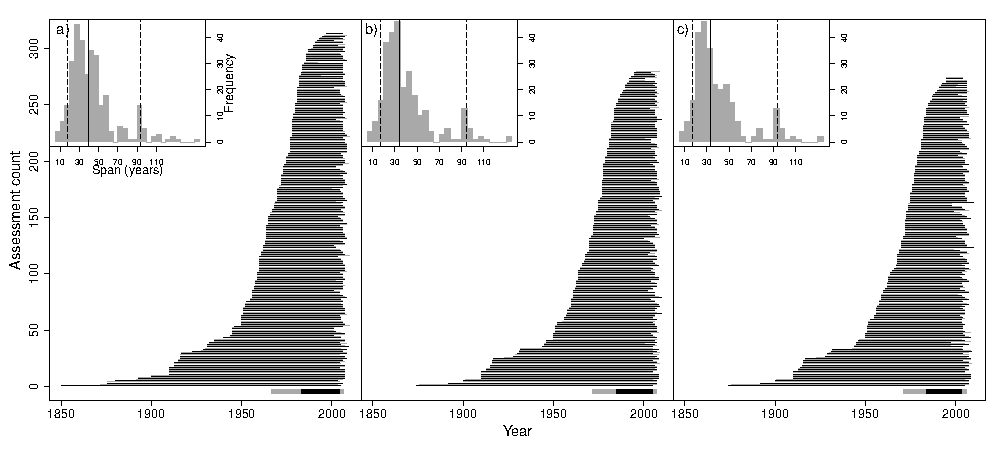
\includegraphics[width=8in]{/home/srdbadmin/srdb/projects/fishandfisheries/R/first-review/orca-plot.pdf}
\end{center}
\caption{ }\label{fig:orca}
\end{figure}
\end{landscape}

\begin{landscape}
\begin{figure}
\begin{center}
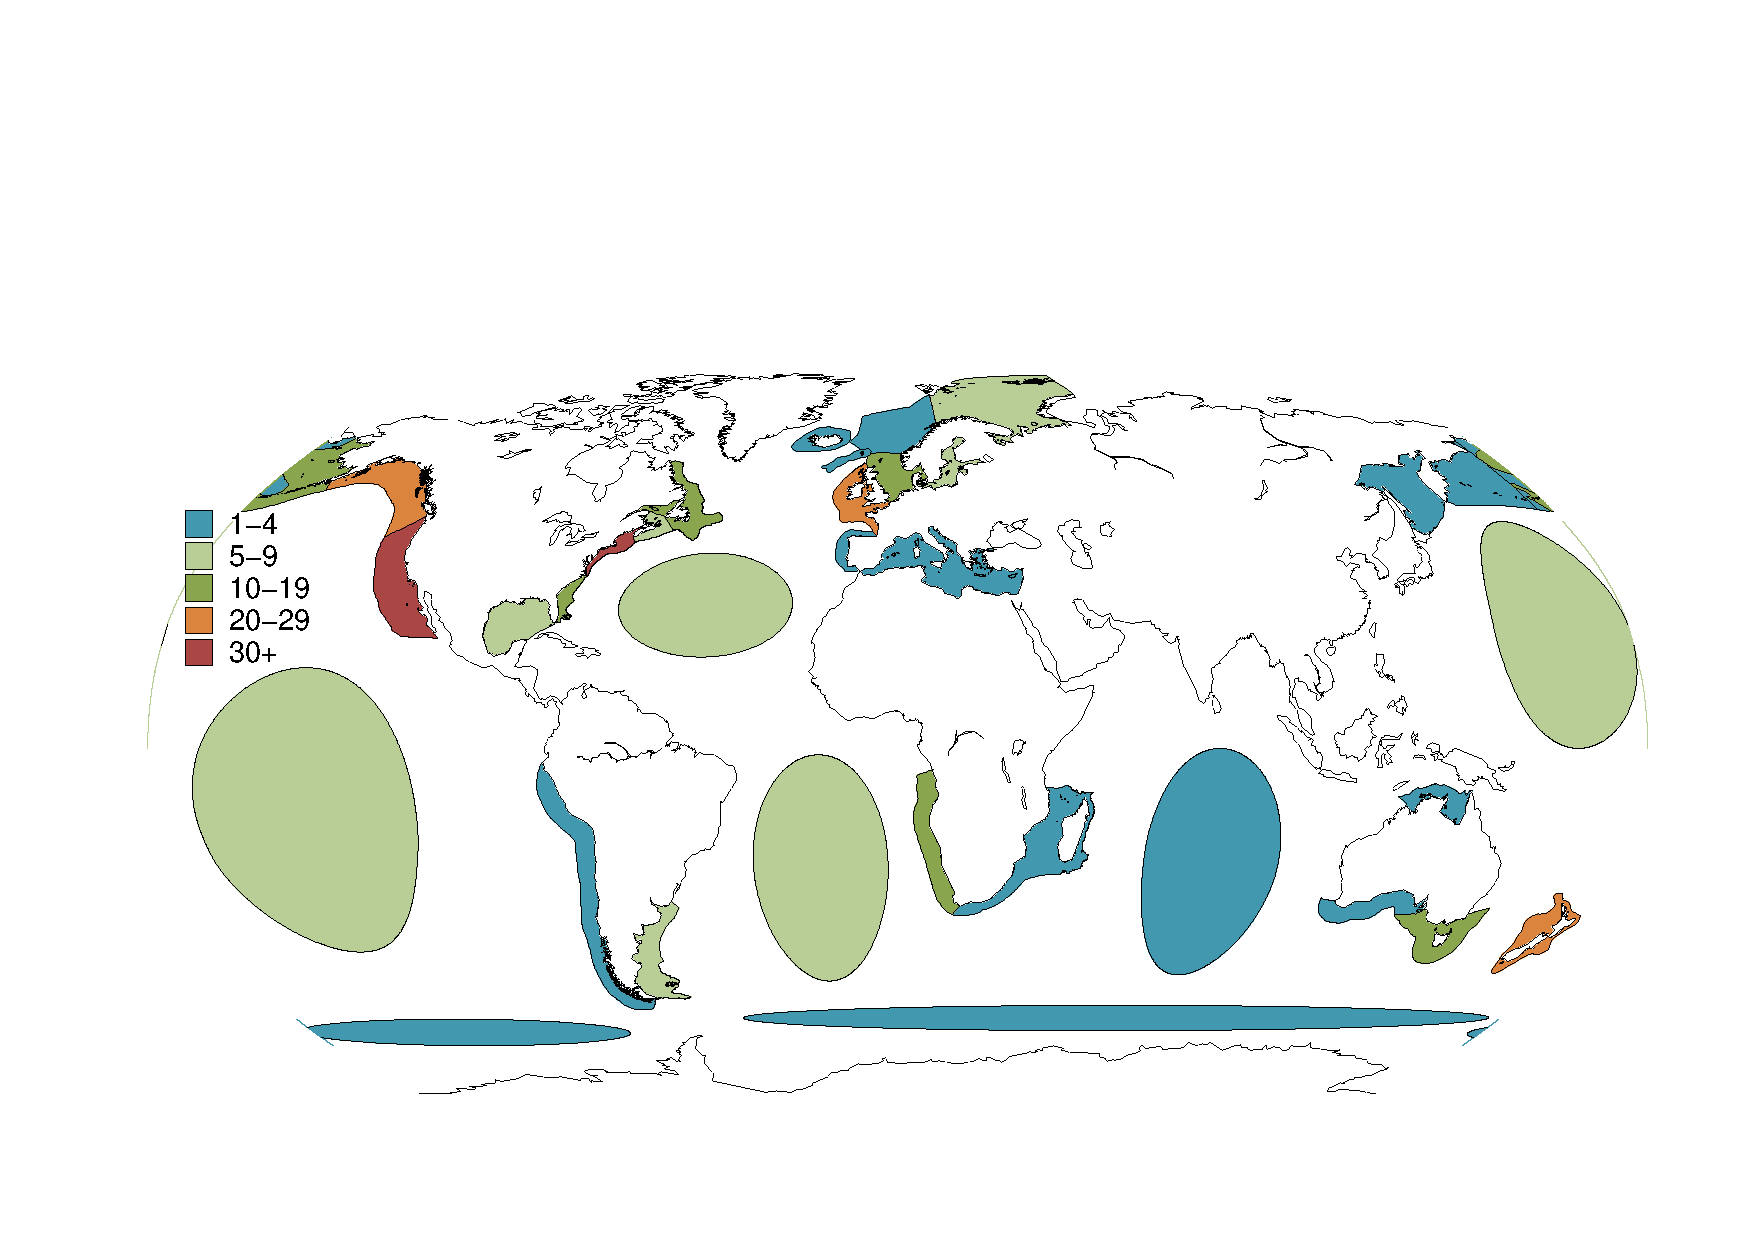
\includegraphics[width=9in]{/home/srdbadmin/srdb/projects/fishandfisheries/GMT/stocks-byLME.pdf}
\end{center}
\caption{ }\label{fig:lmes}
\end{figure}
\end{landscape}


\begin{figure}
\begin{center}
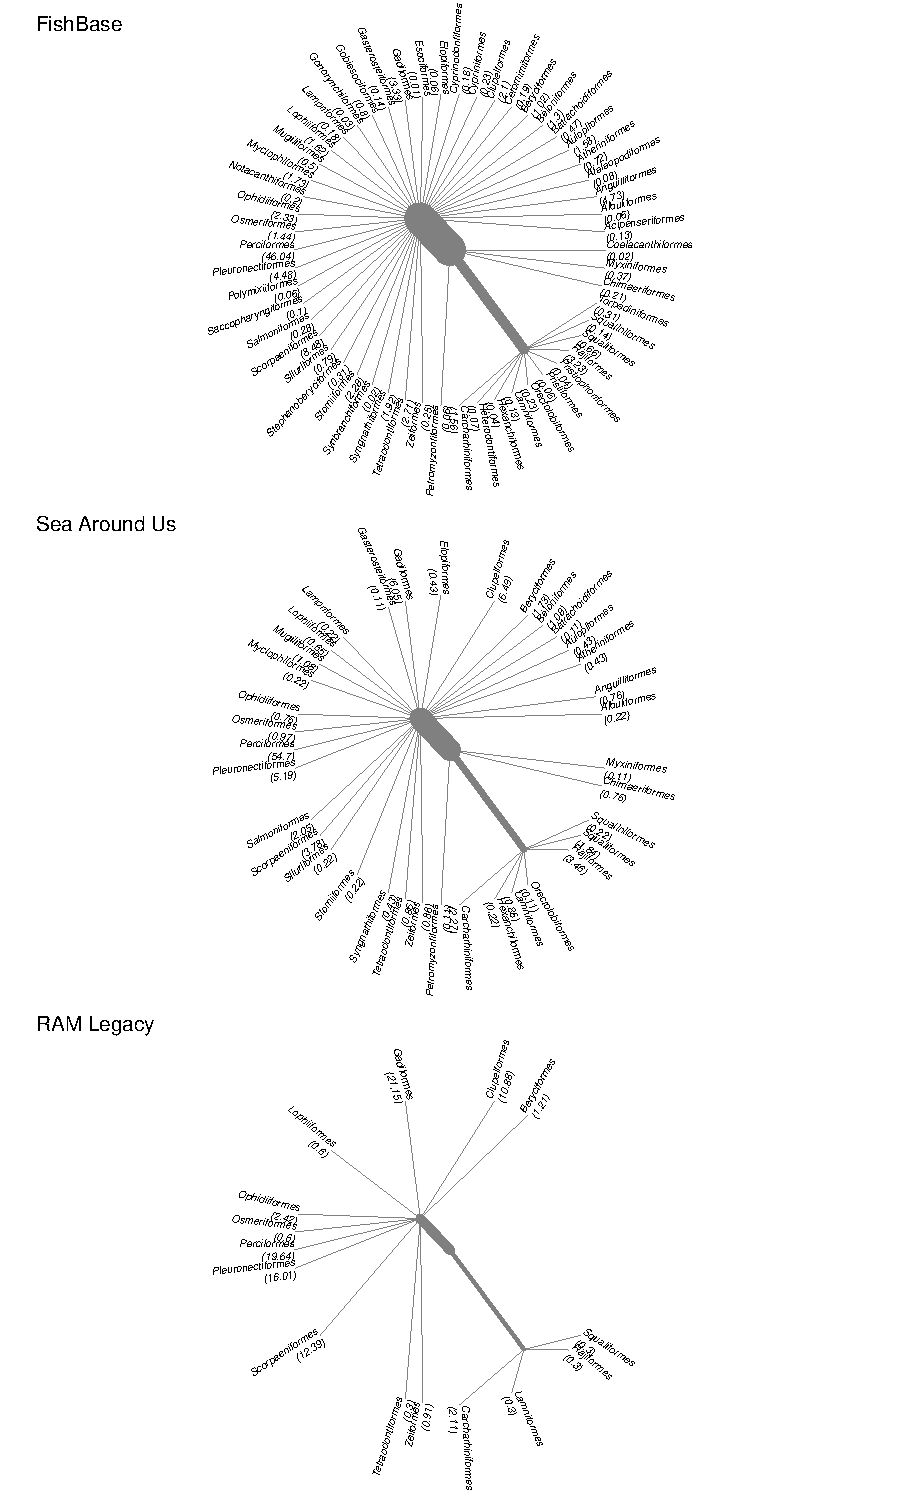
\includegraphics[height=8.5in]{/home/srdbadmin/srdb/projects/fishandfisheries/R/first-review/three-panel-phylo.pdf} % fishbase_saup_two_panel_phylo.pdf}
\end{center}
\caption{ }\label{fig:taxo:threepanel}
\end{figure}




%\begin{figure}
%\begin{center}
%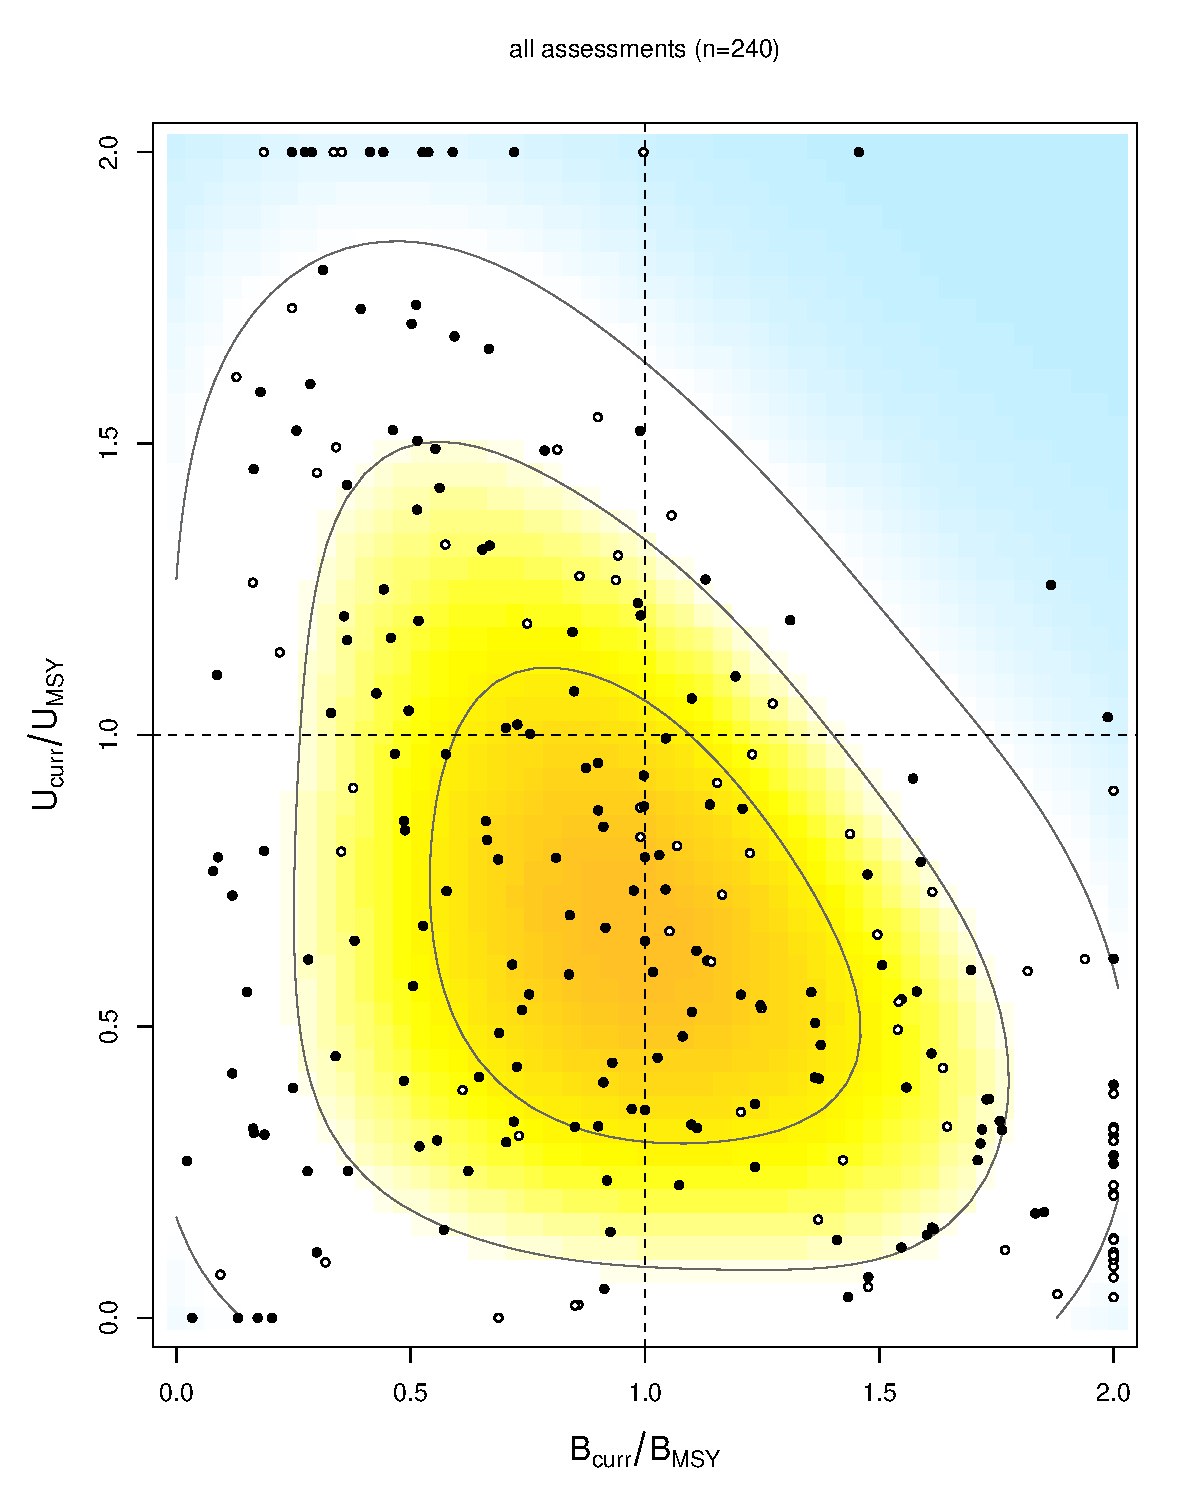
\includegraphics[width=15cm]{/home/srdbadmin/srdb/projects/fishandfisheries/R/first-review/friedegg-single.pdf}
%\end{center}
%\caption{ }\label{fig:friedegg}
%\end{figure}

%Some options for the management-level fried eggs.

%\begin{figure}
%\begin{center}
%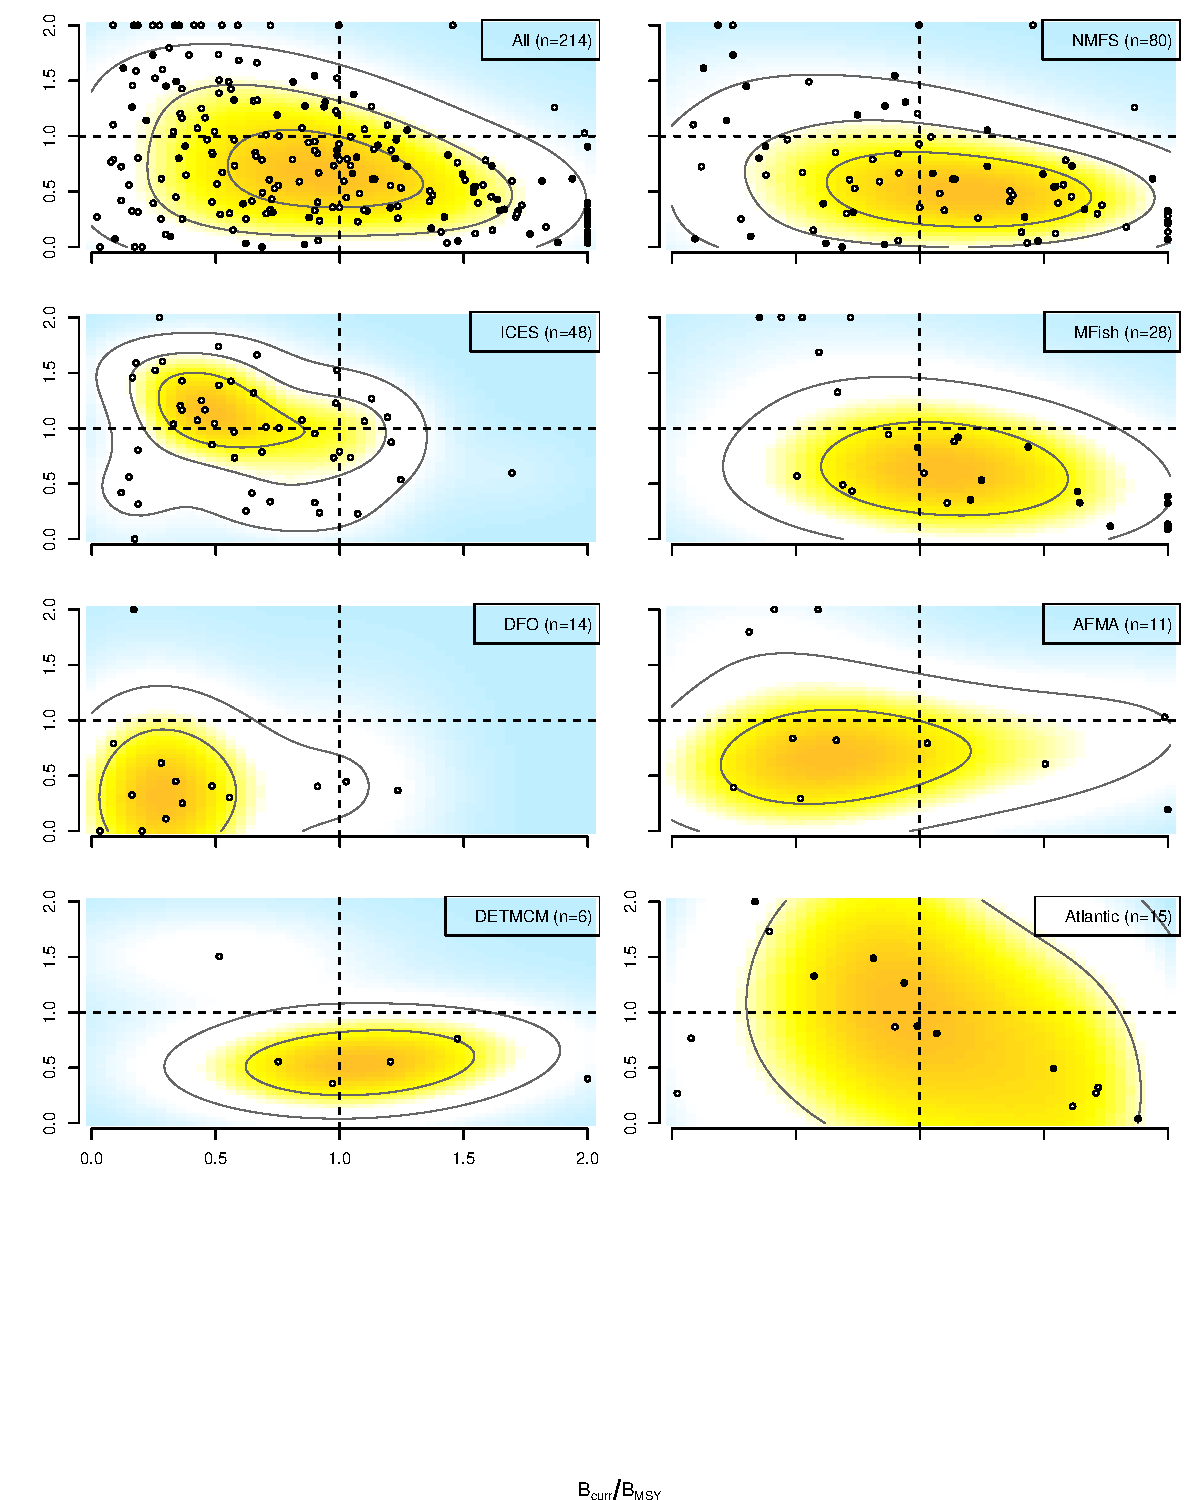
\includegraphics[width=15cm]{/home/srdbadmin/srdb/projects/fishandfisheries/R/first-review/friedegg-bymgmt.pdf}
%\end{center}
%\caption{Option 1 }\label{fig:friedegg}
%\end{figure}

%\begin{figure}
%\begin{center}
%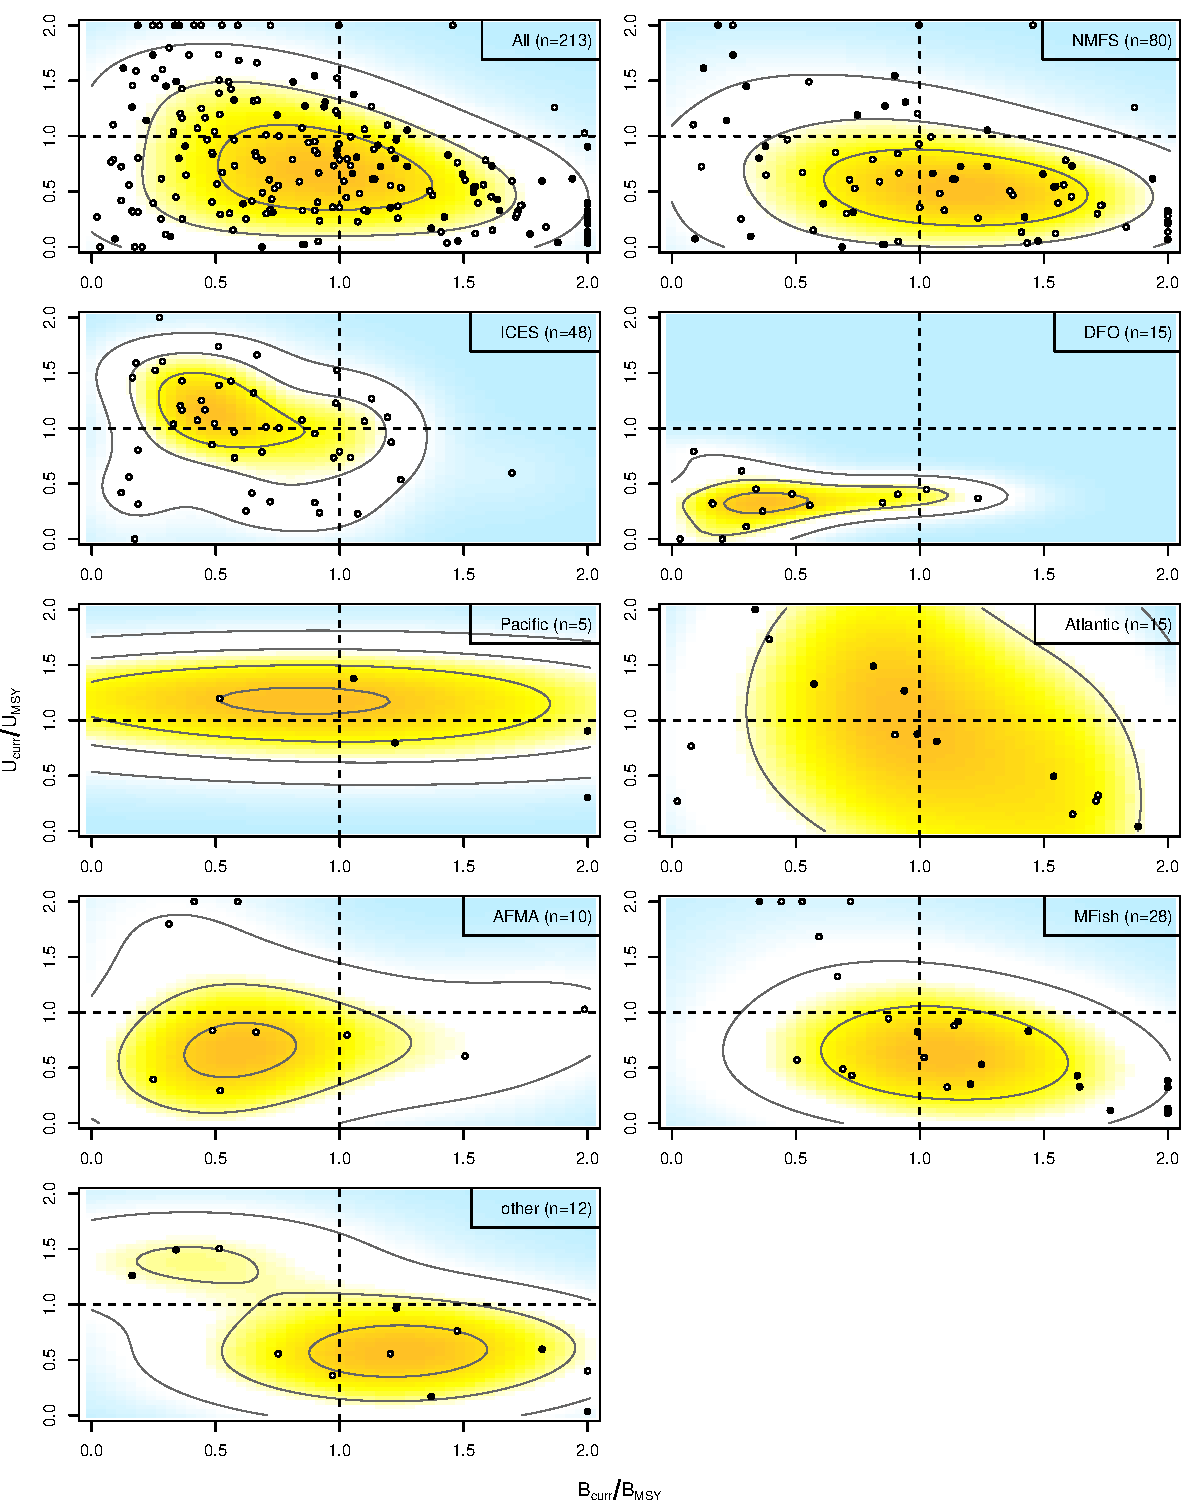
\includegraphics[width=15cm]{/home/srdbadmin/srdb/projects/fishandfisheries/R/first-review/friedegg-bymgmt-10plots.pdf}
%\end{center}
%\caption{Option 2 }
%\end{figure}

%\begin{landscape}
%\begin{figure}
%\begin{center}
%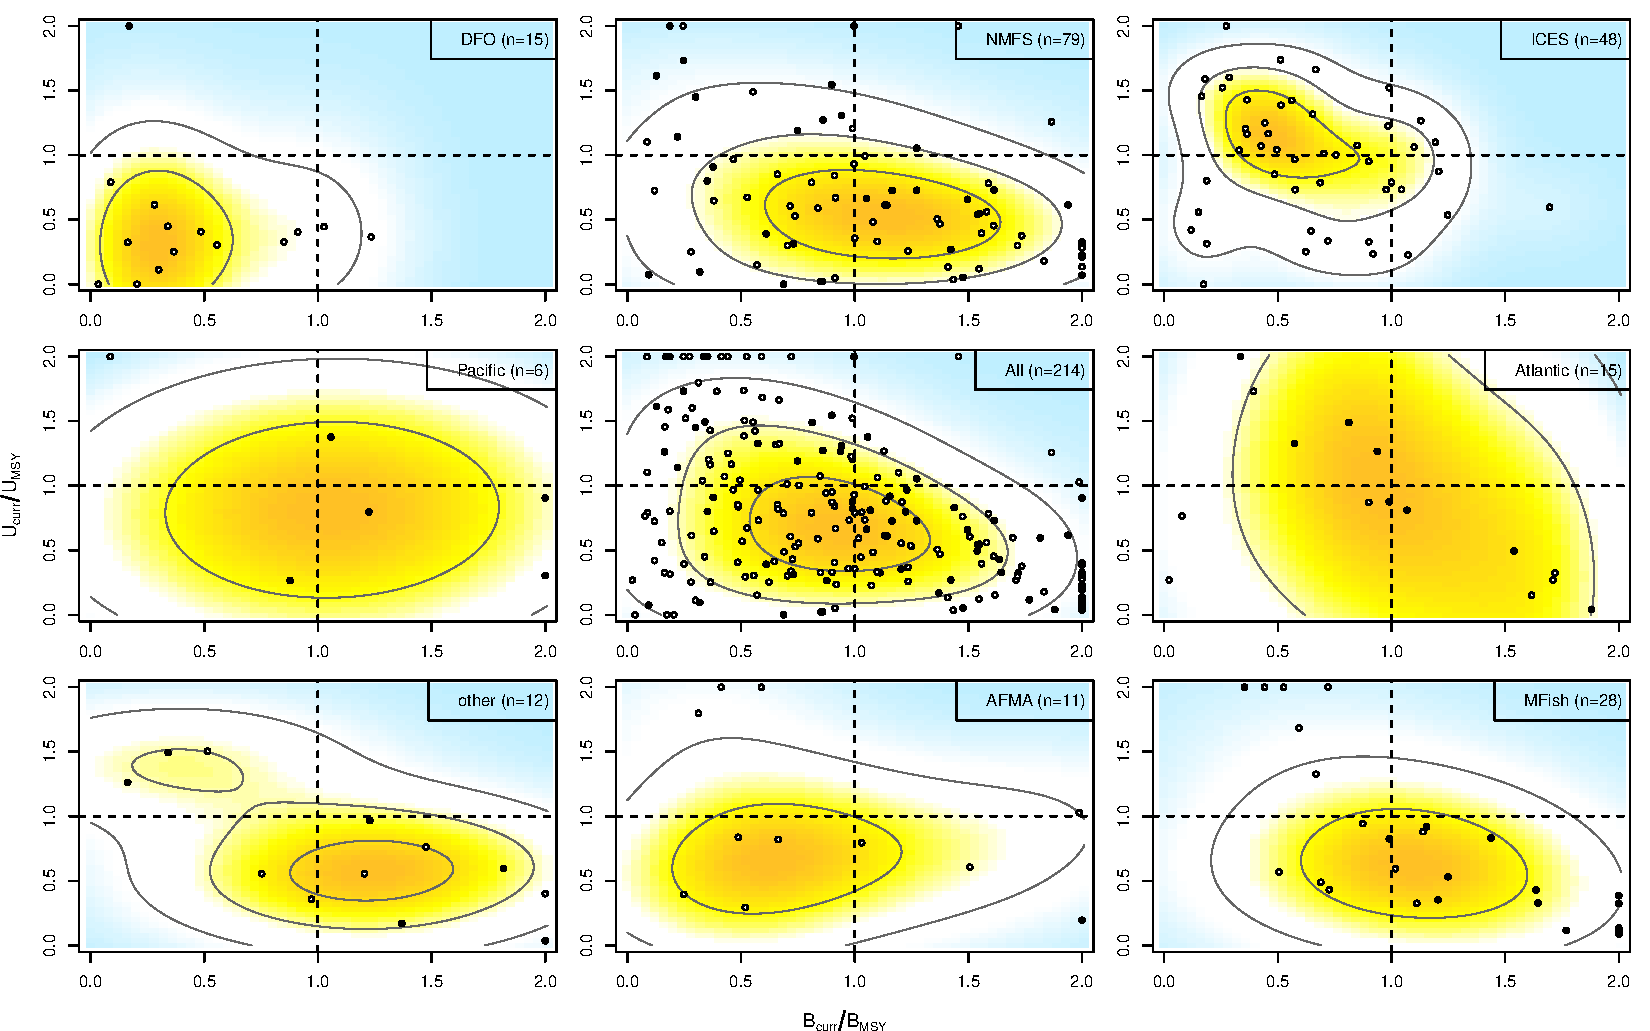
\includegraphics[width=9in]{/home/srdbadmin/srdb/projects/fishandfisheries/R/first-review/friedegg-9plots.pdf}
%\end{center}
%\caption{ Option 3}\label{fig:friedegg}
%\end{figure}
%\end{landscape}

\begin{landscape}
\begin{figure}
\begin{center}
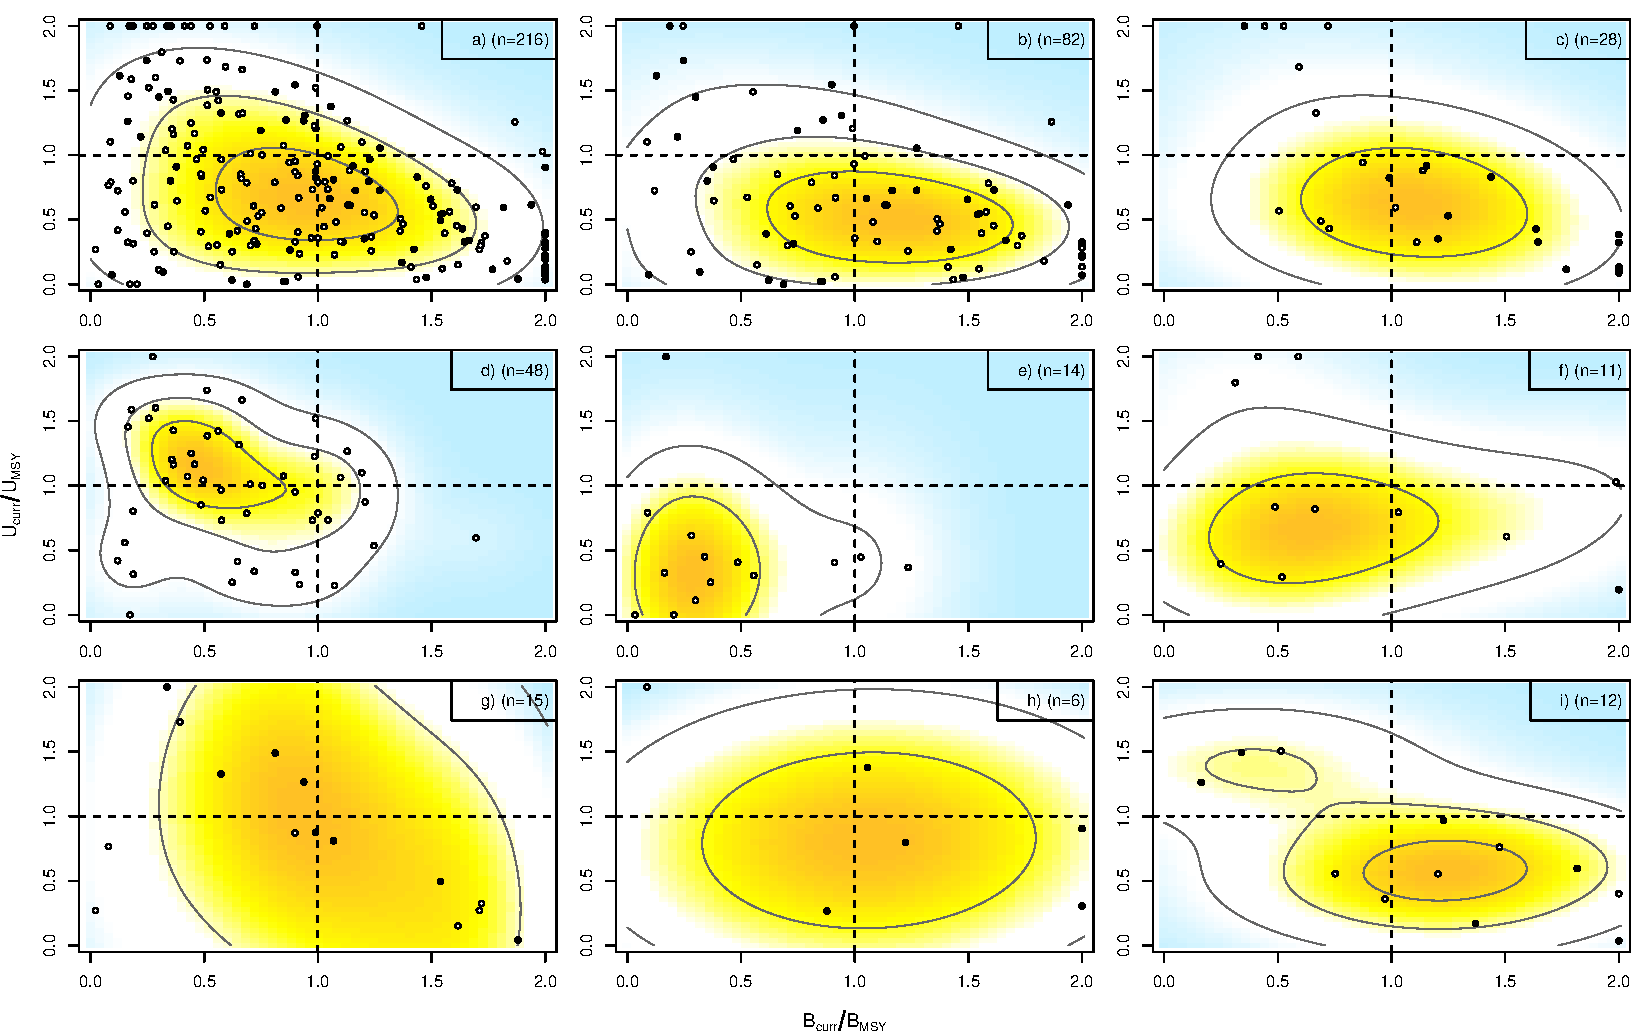
\includegraphics[width=9in]{/home/srdbadmin/srdb/projects/fishandfisheries/R/first-review/friedegg-9plots-fandf.pdf}
\end{center}\label{fig:friedegg}
%\caption{ Option 3}
\end{figure}
\end{landscape}

%For the top 6 taxonomic orders (Figure~\ref{fig:taxo}).
\begin{figure}
\begin{center}
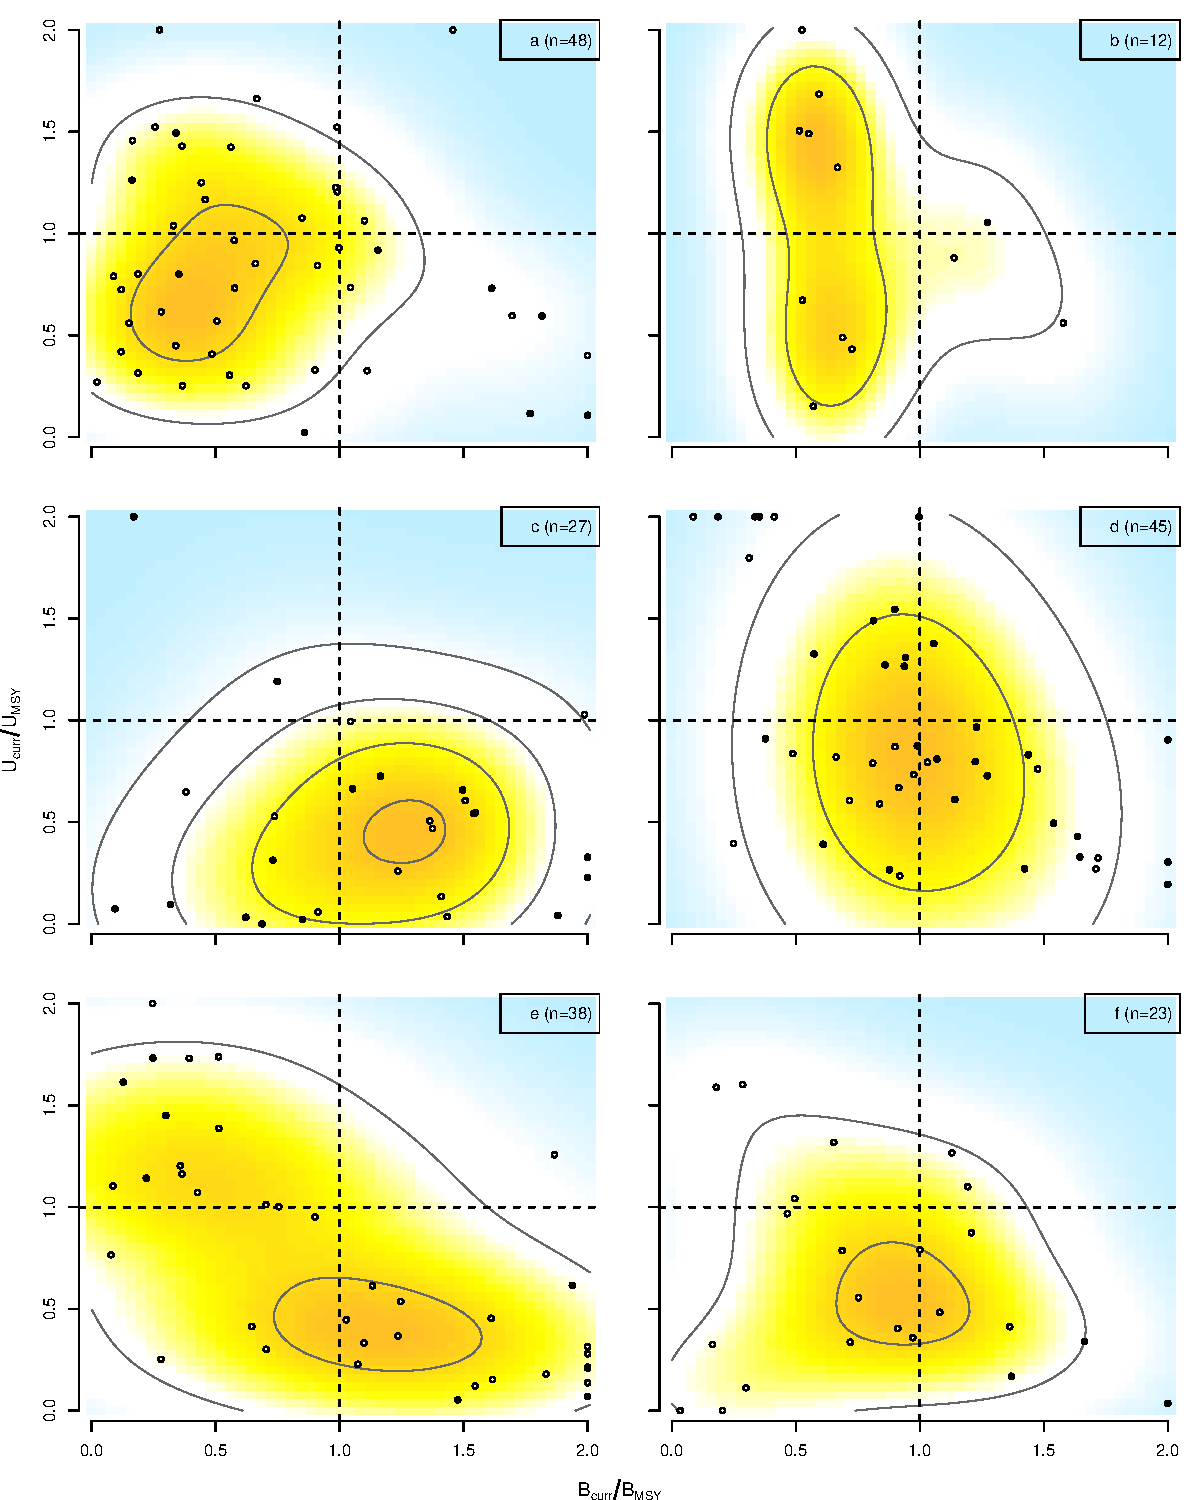
\includegraphics[width=15cm]{/home/srdbadmin/srdb/projects/fishandfisheries/R/first-review/friedegg-taxo.pdf}
\end{center}
\caption{Top 6 taxonomic orders. }
\label{fig:taxo}
\end{figure}

%By trophic level (Figure~\ref{fig:mtl}).
\begin{figure}
\begin{center}
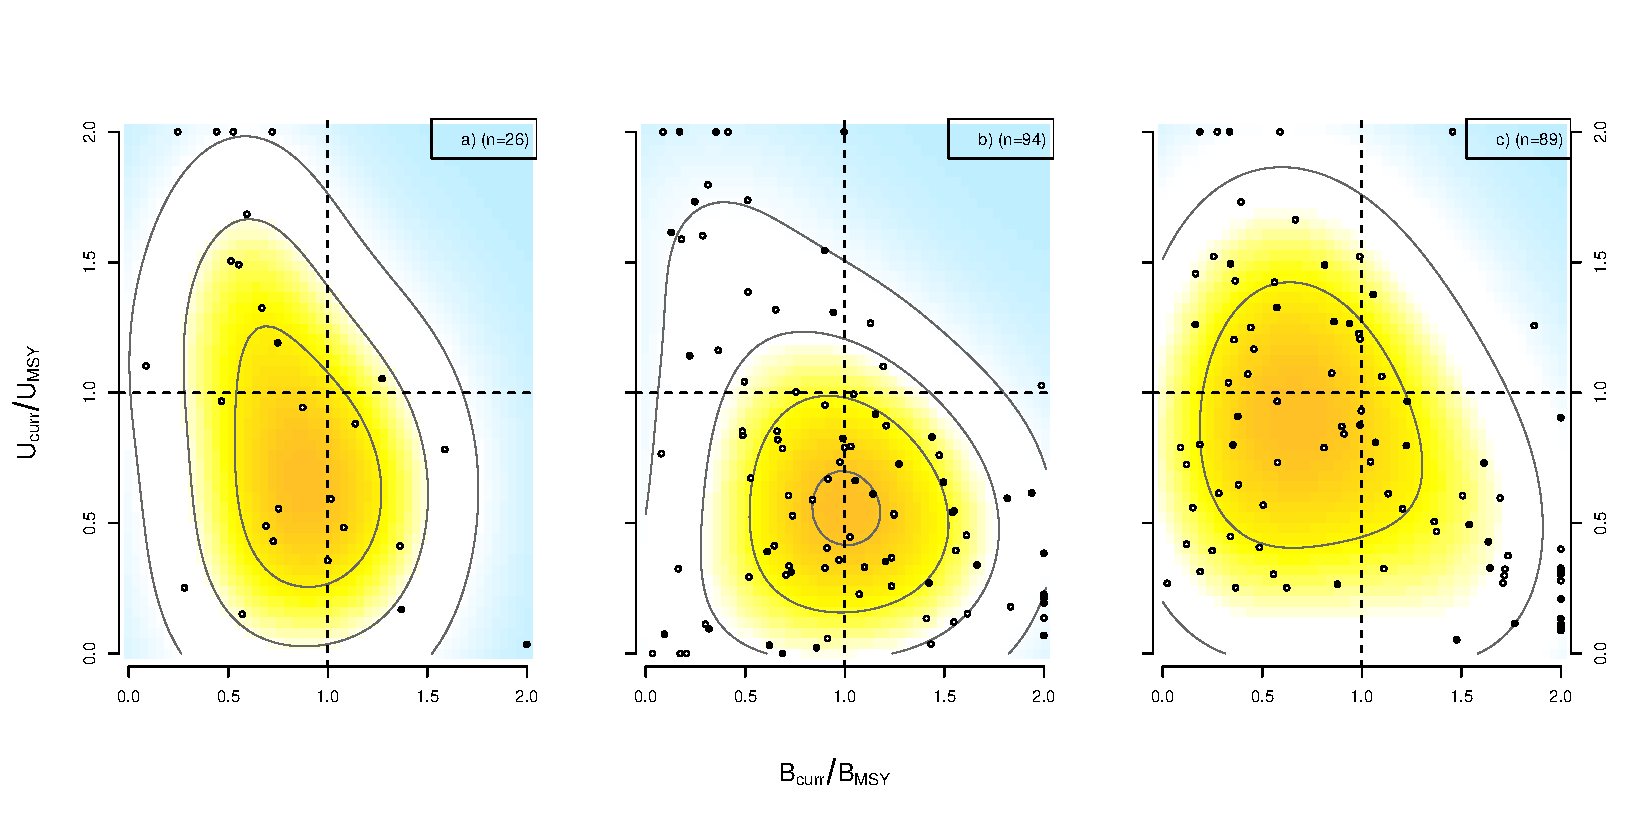
\includegraphics[width=15cm]{/home/srdbadmin/srdb/projects/fishandfisheries/R/first-review/friedegg-MTLs.pdf}
\end{center}
\caption{By mean trophic level (MTL).}
\label{fig:mtl}
\end{figure}







\end{document}

